\documentclass[12pt, twoside]{article}

\usepackage{times,sdtftr}
\usepackage{graphicx,epsfig}        % standard LaTeX graphics tool

\title{Galactik Wars\\ A "MultiPlayer"/"SinglePlayer" third person shooter spaceship game \\Primeira Parte}
\author{Ricardo Alexandre\\ Gon\c{c}alo Amador\\
Universidade da Beira Interior \\
% Place other locations here if you need them by uncommenting
% the following lines.
%\\
%Atomic Computer \& Engineering Facility \\
%Las Vegas NV, 034343\\
}

% Change to the current month of the series
\reportmonth{Junho}
% Change to the current year of the series
\reportyear{2008}
% Change to the TR number that you obtained from the
% UWEETR web pages when you initially created a new
% TR number. Only provide the last 4 digits here, the year
% goes in the \reportyear{} field above.
\reportnumber{10}


\begin{document}
% This first line makes the cover page, which prints the TR number.
\makecover
\blankpage


% This second line makes the title portion of the first page.
\maketitle
\blankpage

\begin{abstract}
\begin{minipage}{1\linewidth}
A toler\^ancia a falhas \'e uma \'area cr\'itica num mundo cada vez mais dependente de sistemas inform\'aticos. 
Neste trabalho abordamos os jogos, a mais abranjente das \'areas da inform\'atica. Nestes est\~ao 
presentes campos como Computa\c{c}\~ao Gr\'afica, Anima\c{c}\~ao e Realidade Virtual, Intelig\^encia Artificial, 
Teoria da Computa\c{c}\~ao, Seguran\c{c}a Inform\'atica, Sistemas Distr\'ibuidos e Toler\^ancia a falhas e Redes.
Este trabalho consiste na implementa\c{c}\~ao de um prot\'otipo de jogo em rede (Primeira Parte) e na 
implementa\c{c}\~ao de t\'ecnicas de toler\^ancia a falhas estudadas no decorrer da cadeira (Segunda Parte). 
\end{minipage}
\end{abstract}
\blankpage


\section{Introdu\c{c}\~ao} 
\begin{minipage}{0.9\linewidth}
O objectivo deste trabalho \'e a implementa\c{c}\~ao de um prot\'otipo de um jogo recorrendo \'a framework (da Microsoft) 
XNA, este jogo dever\'a funcionar em rede ("MultiPlayer" ou "System Link") e em modo jogador \'unico ("SinglePlayer").  
Note-se que nunca foi o nosso objectivo ter um jogo em "Single Player" elaborado, apesar de termos adicionado o m\'aximo de funcionalidades poss\'iveis (referidas 
posteriormente em maior detalhe), n\~ao temos nenhuns modos de jogo. Isto verifica-se, pois o pretendido por n\'os com a 
parte de "SinglePlayer" era a aquisi\c{c}\~ao de conhecimentos que necessit\'avamos para conseguirmos ter a vers\~ao 
"MultiPlayer" a funcionar. Nesta por sua vez temos um modo de competi\c{c}\~ao simples. Temos portanto um prot\'otipo  
de um pot\^encial jogo, uma vez que era invi\'avel criar um jogo elaborado num t\~ao curto espa\c{c}o de tempo (para se 
ter uma ideia um jogo de telem\'ovel leva entre 3 a 4 meses), com a quantidade de pessoas envolvidas (2 pessoas face uma 
equipa de pelo menos 10 pessoas). Apercebemo-nos na primeira apresenta\c{c}\~ao em que fal\'amos do que pretendia-mos 
do nosso trabalho que isto n\~ao era t\~ao transparente aos nossos colegas como a n\'os, pelo que referimos fortemente este ponto antes de prosseguir. 
Ainda a este respeito, a fim de frisar ainda mais esta considera\c{c}\~ao, nos cr\'editos temos vers\~ao "ALPHA" ao 
inv\'es de "BETA" (tendo esse nome sido colocado inicialmente por brincadeira), designa\c{c}\~ao cuja import\^ancia 
constat\'amos que jamais deve ser levada de animo leve. \\
Neste relat\'orio indicamos o que temos j\'a feito e o que pretendemos adicionar na segunda parte. No modo de jogo em 
rede pretendemos acrescentar o m\'aximo de t\'ecnicas de toler\^ancia a falhas poss\'iveis, que sejam pertinentes para 
um jogo, dentro da categoria em que este prot\'otipo se enquadra (Jogo de ac\c{c}\~ao na terceira pessoa). 
Este trabalho serviu para nos iniciar na linguagem C\# e aplicar os conhecimentos que assimil\'amos ao longo da 
licenciatura nas diversas \'areas, j\'a referidas (no abstracto). No entando de frisar que Intelig\^encia Artificial e
Seguran\c{c}a s\~ao campos que descur\'amos, mas que para o resultado deste trabalho se poder designar efectivamente de 
jogo dever\~ao ser tomados em conta.
Nas sec\c{c}\~oes seguintes debru\c{c}amo-nos sobre (por esta ordem) as ferramentas utilizadas, as funcionalidades 
implementadas e as que queremos implementar, a arquitectura e funcionamento do jogo em rede e algumas conclus\~oes que 
ach\'amos pertinetes de reter.
\end{minipage}
\blankpage


\section{Ferramentas ultilizadas}
\begin{itemize}
\begin{minipage}{1\linewidth}
\item .Net Framework 2.0 ou superior - Esta framework da Microsoft \'e actualmente o pilar base de toda a 
aplica\c{c}\~ao desenvolvida em Visual Studio para a Web. Independentemente de se \'e um jogo, um "web-service", etc
nesta framework a Microsoft faculta um pacote de m\'etodos e bibliotecas para todas as funcionalidades pertinentes 
(ou que eles acharam) necess\'arias para este fim. Suporta todas as linguagens desenvolvidas pela Microsoft (VC++,
VB, C\#). No nosso caso temos a vers\~ao 3.5 que \'e uma extens\~ao \'a vers\~ao 2.0, que por sua vez extendeu a 
vers\~ao 1.1.

\item Visual Studio 8 - IDE para desenvolvimento de c\'odigo da Microsoft, sobre a qual o XNA corre. Este c\'odigo 
pode ser desde aplica\c{c}\~oes robustas at\'e web-services. Utiliz�mos a vers\~ao completa no nosso caso (uma vez que 
temos licen\c{c}a), no entanto a vers\~ao express (gratuita com algumas limita\c{c}\~oes) teria sido suficiente (ver 
quadro comparativo em http://msdn.microsoft.com/en-us/vs2005/aa700921.aspx para uma ideia mais detalhada). 

\item SpaceWar - Exemplo de aprendizagem de onde retir\'amos grande parte dos efeitos son\'oros e modelos que 
utiliz\'amos no nosso prot\'otipo de jogo. Distribuido para fins de aprendizagem, n\~ao possui modo em rede mas possui 
"MultiPlayer".

\item Blender - Ferramenta gratuita para anima\c{c}\~ao e modela\c{c}\~ao 3D, us\'amo-la para fazer o modelo do escudo. 
Esta ferramenta permite exportar em formato .x (DirectX format), que \'e o formato de modelos 3d que o XNA suporta.
\end{minipage}
\end{itemize}
\blankpage

\begin{itemize}
\begin{minipage}{1\linewidth}
\item XNA Framework 2.0 - Framework especificamente criada para o desenvolvimento de jogos para Windows ou XBOX 360, 
usando a linguagem C\#. Desenhada utilizar os recursos do Microsoft Visual C\#, esta framework apoia-se sobre a 
t\'ecnologia DirectX e a plataforma .Net. Permite a manipula\c{c}\~ao/edi\c{c}\~ao de som com uma ferramenta pr\'opia 
(XACT), importa\c{c}\~ao de modelos e texturas, entre outras caracter\'isticas pertinentes ferramentas de 
desenvolvimento de jogos. Estende a plataforma .Net, e tem para os modos de jogo em rede suporte ao servi\c{c}o de 
jogos do Live e de sess\~oes "System Link" (liga\c{c}\~ao entre m\'aquinas dentro de uma rede local).\\ 
O XNA tem uma componente designada de "Content Pipeline", sendo o respons�vel por converter (quando \'e feito o "build") 
os formatos suportados em formatos reconhecidos durante a execu\c{c}\~ao. Os formatos que podem ser usados s\~ao 
limitados, e no XNA 3.0 (lan\c{c}amento previsto para o ver\~ao de 2008) alguns v\~ao deixar de ser suportados (ainda 
n\~ao est\~ao definidos quais explicitamente). Actualmente s\~ao suportados os seguintes formatos:
\begin{itemize}
\begin{minipage}{1\linewidth}
\item Ficheiros 3D (Modelos): .FBX e .X

\item Ficheiros 2D (Texturas): .BMP, .JPG, .PNG e .TGA

\item Audio: .wav, .aif, .aiff (estes 3 representam os formatos de audio que podemos colocar num projecto do XACT), 
	.XAP (gestor de conte\'udo audio nos formatos j\'a indicados XACT)
 
\item Ficheiros de informa\c{c}\~ao (Materiais e Dados) - .FX e .XML (este segundo atrav\'es das funcionalidades do 
	Visual C\#)  

\end{minipage}
\end{itemize}
\end{minipage}
\end{itemize}
\blankpage


\section{Funcionalidades}
\begin{minipage}{1\linewidth}
Tal como j\'a foi referido o nosso objectivo \'e criar um prot\'otipo de jogo.  
De seguida indicamos as funcionalidades, e o respectivo estado de implementa\c{c}\~ao destas, que pretendemos do nosso 
c\'odigo. Posteriormente falamos destas mais detalhadamente. \\
\begin{itemize}
\begin{minipage}{1\linewidth}
\item Funcionalidades Primeira Parte:
\begin{itemize}
\begin{minipage}{1\linewidth}
\item Sistema de menus. (Implementado)

\item Op\c{c}\~oes de regula\c{c}\~ao de som (audio e efeitos). (Implementado)

\item Modo Single Player. (Implementado)

\item Modo "MultiPlayer". (Implementado)

\item Fundo m\'ovel e m\'ultiplos cen\'arios de fundo. (Implementado)

\item Sistema de particulas. (Em fase de Implementa\c{c}\~ao)

\item C\^amara gen\'erica. (Implementado)
\end{minipage}
\end{itemize}

\item Funcionalidades Segunda Parte:
\begin{itemize}
\begin{minipage}{1\linewidth}
\item Pontua\c{c}\~ao em jogo "MultiPlayer". (Em fase de Implementa\c{c}\~ao)

\item Migra\c{c}\~ao do Host se este cair. (Em fase de Implementa\c{c}\~ao)

\item Manuten\c{c}\~ao do estado de um dos jogadores se este cair, por um tempo m\'inimo. 
(Em fase de Implementa\c{c}\~ao)

\item Permitir a um cliente aderir a uma sess\~ao se esta ainda decorrer. (Em fase de Implementa\c{c}\~ao)

\item Predic\c{c}\~ao de enventos. (Em fase de Implementa\c{c}\~ao)
\end{minipage}
\end{itemize}
\end{minipage}
\end{itemize}
\end{minipage}

\subsection{Funcionalidades Primeira Parte}
\begin{minipage}{1\linewidth}
Estas s\~ao as bases para termos o nosso (prot\'otipo de) jogo a funcionar, e para futuramente este poder ser estendido 
(fora do \^ambito da cadeira) a um demo funcional e quem sabe a um jogo completo.
\end{minipage}

\subsubsection{Sistema de menus}
\begin{minipage}{1\linewidth}
Existe um sistema de menus j\'a feito para jogos de rede ou s\'o "SinglePlayer". Fizemos o download deste, e
tentou-se perceber o c\'odigo o melhor poss\'ivel, sem documenta\c{c}\~ao, e estendeu-se/alterou-se conforme o 
pretendido para o caso a aplicar. 
No nosso caso acrescent\'amos as sec\c{c}\~oes "credits" e "options". O menu est\'a actualmente implementado e a 
funcionar, n\~ao alteramos o aspecto gr\'afico deste, somente nos preocup\'amos em implementar os menus referidos.\\
A imagem seguinte explica o que \'e poss�vel fazer no sistema de menus:
\end{minipage}
\begin{figure}[htp]
\centering
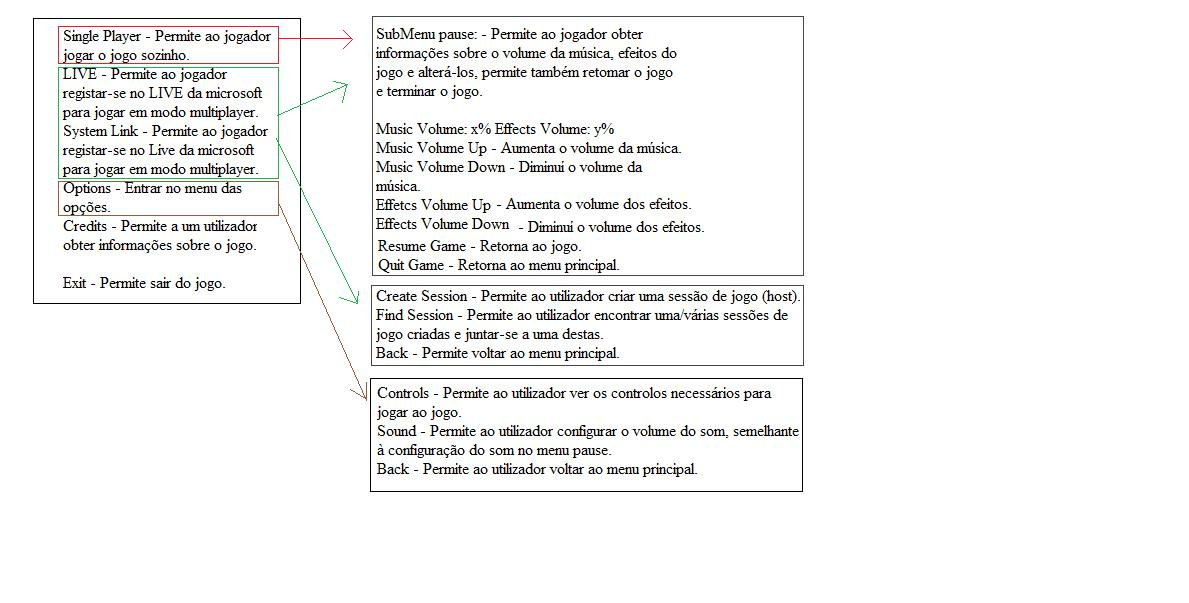
\includegraphics[scale=0.6]{images/Menu.jpg}
\caption{Funcionalidades do Sistema de Menus.}
\end{figure}

\subsubsection{Op\c{c}\~oes de regula\c{c}\~ao de som (audio e efeitos)}
\begin{minipage}{1\linewidth}
Dentro do menu por n\'os adicionado ("options"), podemos regular o som da m\'usica de fundo e os efeitos especiais.
Isto tamb\'em pode ser feito nos modos de jogo, quando pausamos o jogo (em rede n\~ao pausamos o jogo quando 
premimos a tecla "Escape", tal como nos FPS em rede aparece o menu mas o jogo continua a funcionar, pois n\~ao faz 
sentido um dos clientes poder parar o jogo a todos os outros jogadores por tempo indeterminado), para o efeito 
acrescent\'amos uma nova funcionalidade, al\'em das que existiam, quando o jogo se encontra em "pause", para regular 
audio e efeitos sonoros. Adicion\'amos al\'em dos sons retirados do kit de treino conhecido por "SpaceWar" (de onde 
retir\'amos os nossos modelos e efeitos son\'oros) uma compila\c{c}\~ao de v\'arias m\'usicas para m\'usica de fundo.\\
Algumas notas, no XNA o som \'e suportado no formato wave outros formatos s\~ao utilizados de forma n\~ao nativa via
"Content Pipeline". Este mecanismo funciona como um interpretador de determinados formatos para a\'udio (.wav), 
objectos (.x), texturas (.png, .tga), para um c\'odigo m\'aquina a ser corrido pela m\'aquina virtual do C\#.
No nosso trabalho temos uma classe, feita por n\'os, que tem os m\'etodos necess\'arios a manipula\c{c}\~ao do som 
("SoundHandler.cs"). Temos um bug na manipula\c{c}\~ao do som na parte de rede que constat\'amos, para o qual ainda 
n\~ao existe uma solu\c{c}\~ao divulgada, mas que tent\'amos por v\'arias formas resolver sem sucesso. Este problema 
devesse a uma limita\c{c}\~ao na ferramenta de controlo de listas de a\'udio ("Cues") e suas respectivas propriedades 
(o som toca em loop, nome da faixa, etc) utilizada no XNA (XACT). Estamos no entanto ainda a tentar ver se existe alguma 
alternativa que n\~ao tenhamos experimentado que resolva este problema, motivo pelo qual em rede s\'o a nossa nave faz
barulho quando se desloca. 
De seguida uma pequena amostra de c\'odigo essencial pertinente para manipular som no XNA: \\
\end{minipage}

\begin{itemize}
\begin{minipage}{1\linewidth}
\item Cria\c{c}\~ao dos objetos\\
AudioEngine audioEngine;\\
WaveBank waveBank;\\
SoundBank soundBank;\\
protected override void Initialize()\{ \\
audioEngine = new AudioEngine("MySounds.xgs"); \\
waveBank = new WaveBank(audioEngine, "Wave Bank.xwb"); \\
soundBank = new SoundBank(audioEngine, "Sound Bank.xsb"); \\
base.Initialize(); \\
\} 

\item Gerar um efeito sonoro (som sem loop)\\
soundBank.PlayCue("chord");

\item Tocar m\'usica de fundo (som com loop)\\
// Iniciar a m\'usica \\
myLoopingSound = soundBank.GetCue("notify"); \\
myLoopingSound.Play(); \\
// Parar ou continuar a m\'usica \\
if (myLoopingSound.IsPaused) \\
myLoopingSound.Resume(); \\
else \\
myLoopingSound.Pause();
\end{minipage}
\end{itemize}
 
\subsubsection{Modo "SinglePlayer"}
\begin{minipage}{1\linewidth}
Neste modo seguimos um tutorial online para fazer um jogo tipo "asteroids". Ap\'os este estar conclu\'ido 
acrescent\'amos algumas extras (rockets, escudo) e migr\'amos o c\'odigo para o nosso sistema de menus 
(classe pr\'opria para o jogo chamada "GamePlayScreen.cs"). O jogo neste modo tem uma dificuldade crescente, que 
conciste no aumento da velocidade dos asteroides quando estes s\~ao restaurados, ap\'os a destrui\c{c}\~ao de todos os 
asteroides que j\'a existiam (n\'umero regul\'avel na classe "GameVariables.cs"). O jogo acaba se o utilizador ap\'os 
perder o escudo bater num meteoro. O valor inicial do escudo e o dano que cada meteoro causa no jogador s\~ao 
vari\'aveis da classe "GameVariables.cs".
Quando isto acontece aparace um menu de "Game Over", com a respectiva musica de fundo. O jogo tem as bases (referidas 
de seguida) para ter um sistema de n\'iveis e inimigos elaborado, mas trata-se de um modo relativamente simples 
actualmente. Temos presente a informa\c{c}\~ao das vidas, escudo restante, asteroides existentes, n\'ivel e 
pontua\c{c}\~ao actual do jogador.
\end{minipage}

\subsubsection{Fundo m\'ovel e m\'ultiplos cen\'arios de fundo}
\begin{minipage}{1\linewidth}
A ideia por detr\'as desta funcionalidade prende-se com potencializar n\'iveis dum tipico shooter de naves. A maioria
dos tradicion\'ais jogos 2D de naves em "SinglePlayer" tem n\'iveis em que o cen\'ario se move. Ao fim de algum tempo 
aparece um inimigo mais forte (Level Boss ou Level Sub Boss seguido mais a frente do anterior), se este for derrotado 
passamos de n\'ivel. O jogo acaba ao fim de determinada quantidade de n\'iveis, ou se perdermos um determinado n\'umero 
de vidas. Esta funcionalidade (fundo m\'ovel) pode ou n\~ao estar activada (controlado pela variav\'el 
"ScrollingBackgroundIsActive" na classe "GameVariables.cs"). Se esta funcionalidade n\~ao estiver activa a classe que 
implementa esta funcionalidade designada "ScrollingBackground.cs" n\~ao \'e criada e \'e feita uma escolha aleat\'oria 
de entre um conjunto de fundos est\'aticos (acrescent\'ados por n\'os), no arranque do jogo.
\end{minipage}

\subsubsection{Sistema de part\'iculas}
\begin{minipage}{1\linewidth}
Esta funcionalidade pretende simular efeitos naturais como por exemplo explos\~oes (quando a nave for destruida), 
rasto das naves (quando estas se deslocam). Existe uma quantidade consider\'avel de outros efeitos interessantes afim de 
tornar um jogo mais interessante, sendo esta funcionalidade algo que nunca implement\'amos mas que j\'a usamos e 
estud\'amos (efeitos de part\'iculas \'e uma das funcionalidades do Blender). \'E um dos componentes mais comuns dos 
motores gr\'aficos actuais. Uma vez que esta funcionalidade n\~ao \'e requerida temo-la como opcional, mas achamos que
temos uma vers\~ao desta a funcionar na entrega da segunda parte.
\end{minipage}

\subsubsection{C\^amara gen\'erica}
\begin{minipage}{1\linewidth}
A c\^amara que usamos actualmente \'e est\'atica, ou m\'ovel se o desejarmos (segue a nave no nosso caso). Como \'e 
comun em muitos tipos de jogos (se n\~ao todos), existe uma classe c\^amara que permite vizualisarmos o jogo de 
determinados \^angulos pretendidos. De notar que este jogo \'e em 3D (os modelos s\~ao 3D mas os cen\'arios n\~ao) mas 
\'e visto em 2D (de cima projectado no plano), pelo que o jogo poderia ter uma vers\~ao 2D (visto de cima) e 3D (visto 
a uma pequena dist\^ancia da parte traseira da nave). A ideia \'e que o jogo seja em 3D ou 2D quase s\'o pela 
altera\c{c}\~ao desta classe ("CCamera.cs"), e com a adi\c{c}\~ao das considera\c{c}\~oes inerentes a um novo grau de 
liberdade (movimento dos objectos detec\c{c}\~ao de colis\~oes, etc). Os controlos estendidos ao 3D s\~ao um trabalho 
que poder\'a ser feito posteriormente \'a conclus\~ao da cadeira.
\end{minipage}

\subsubsection{Modo "MultiPlayer"}
\begin{minipage}{1\linewidth}
Neste modo, no sistema de menus, j\'a tinhamos a parte da cria\c{c}\~ao de sess\~oes tratada; a parte da toler\^ancia a 
falhas n\~ao se encontra aqui tratada, ficando ao nosso crit\'erio o que queremos fazer e como o vamos fazer.\\
O que n\'os temos \'e o nosso prot\'otipo de jogo a funcianar em "MultiPlayer" dentro de uma rede (lan local e n\~ao 
sobre a internet). Temos uma sess\~ao em que quem a cria \'e o seu host e os outros utilizadores podem criar a sua 
sess\~ao ou juntar-se a uma j\'a criada. A rede mais em detalhe \'e explicada no proximo cap\'itulo.
Cada sess\~ao local pode ter no m\'aximo 16 jogadores e um sess\~ao em rede pode chegar a 31 jogadores no m\'aximo; no 
nosso caso reduzimos para 6, porque n\~ao tinhamos mais modelos distintos de naves (outra coisa que posteriormente a 
esta cadeira seria interessante de fazer seria criar modelos de naves nossos). \\
Neste modo temos um sess\~ao de at\'e 6 jogadores que lutam entre si o ult\'imo vivo ganha a sess\~ao. Ser\'a mostrada a
sua pontua\c{c}\~ao bem como a dos outros jogadores antes de a sess\~ao terminar. (A implementar na segunda parte)\\
No jogo temos duas entidades um Host e os clientes. Os passos por que estes passam desde o \'inicio ao fim de uma 
sess\~ao encontram-se de seguida descritos.\\
\begin{minipage}{0.4\linewidth}
Passos no Host: \vspace{0.2cm}
\begin{itemize}
\begin{minipage}{1\linewidth}
\item Executar sign-in.
\item Criar Sess\~ao (abrir um "Lobby").
\item Esperar que os jogadores se liguem e informem que est\~ao prontos ("ready").
\item Iniciar jogo (sair do "Lobby" para o jogo).
\item Trocar mensagens durante o jogo.
\item Terminar jogo (sair do jogo). \\
\end{minipage}
\end{itemize}
\end{minipage}
\begin{minipage}{0.4\linewidth}
Passos nos clientes: \vspace{0.2cm}
\begin{itemize}
\begin{minipage}{1\linewidth}
\item Executar sign-in.
\item Procurar uma Sess\~ao com slots dispon\'iveis.
\item Conectar-se \'a sess\~ao (entrar no "Lobby").
\item Informar que se est\'a pronto para iniciar ("ready").
\item Confirmar este estado para saber quando jogo come\c{c}ou e terminou.
\item Trocar mensagens durante o jogo. \\
\end{minipage}
\end{itemize}
\end{minipage}
\end{minipage}

\begin{minipage}{1\linewidth}
O que tivemos de fazer neste modo para o envio de dados, consistiu em recorrer aos m\'etodos de passagem de mensagens 
da plataforma .Net (extendidos no XNA "System.Threading", "Microsoft.Xna.Framework.GamerServices" e 
"Microsoft.Xna.Framework.Net"), para enviar os dados que cada jogador precisa de saber sobre os restantes. 
Estes s\~ao (neste exemplo reduzido):\\
\begin{itemize}
\begin{minipage}{1\linewidth}
\item{\bf{Envio de Mensagens:}} \\

PacketWriter packetWriter = new PacketWriter();	\\	
public void SendMessage(string mensagem) \{ \\ 
foreach (LocalNetworkGamer localPlayer in session.LocalGamers) \{ \\
packetWriter.Write(mensagem); \\
localPlayer.SendData(packetWriter,SendDataOptions.None); \} \} \\

\item{\bf{Recep\c{c}\~ao de Mensagens:}} \\

PacketReader packetReader = new PacketReader(); \\
public string ReceiveMessage() \{ \\
String Mensagem = String.Empty; \\
NetworkGamer remotePlayer; \\
foreach (LocalNetworkGamer localPlayer in session.LocalGamers)  \{ \\
while (localPlayer.IsDataAvailable) \{ \\����������
localPlayer.ReceiveData(packetReader, out remotePlayer); \\
if (!remotePlayer.IsLocal) \\ 
message = packetReader.ReadString(); \} \} \}
\end{minipage}
\end{itemize}
\end{minipage}

\subsection{Funcionalidades Segunda Parte}
\begin{minipage}{1\linewidth}
Das t\'ecnicas de toler\^ancia a falhas pertinetes vistas no decorrer da cadeira, as que se seguem foram as que 
opt\'amos por implementar, se houver alguma extra a adicionar interessante mas vi\'avel no tempo que ainda temos ser\'a 
adicionada ao relat\'ario final.
\end{minipage}

\subsubsection{Pontua\c{c}\~ao em jogo "MultiPlayer"}
\begin{minipage}{1\linewidth}
Esta funcionalidade consiste em mostrar a pontua\c{c}\~ao ordenada (dos que t\^em mais para os que t\^em menos pontos).
N\~ao est\'a implementada porque est\'a ligada a manuten\c{c}\~ao dos estados, a sua visualiza\c{c}\~ao j\'a \'e 
aplic\'avel mas n\~ao se encontra presente enquanto a manuten\c{c}\~ao dos estados n\~ao estiver aplicada. 
\end{minipage}

\subsubsection{Migra\c{c}\~ao do Host se este cair}
\begin{minipage}{1\linewidth}
Para aplicar esta funcionalidade temos uma propriedade dos objectos do tipo "NetworkSession" que assegura que \'e 
realizada a migra\c{c}\~ao do host para um dos clientes presentes na sess\~ao. Ainda nos falta identificar o local 
exacto da cria\c{c}\~ao das sess\~oes para que esta funcionalidade esteja activada. De notar que o nosso jogo funciona 
em P2P sen\~ao esta funcionalidade seria impratic\'avel (num modelo cliente-servidor o servidor seria substituido por 
um de backup mas um cliente seria sempre e somente um cliente)!
\end{minipage}

\subsubsection{Manuten\c{c}\~ao do estado de um dos jogadores se este cair, por um tempo m\'inimo}
\begin{minipage}{1\linewidth}
O que pretendemos nesta funcionalidade \'e que por um tempo determinado por n\'os, se um cliente cair, manter o estado 
deste at\'e que ele retorne ou outro jogador tome o seu lugar. No segundo caso o novo jogadar fica com os dados por 
omiss\~ao e os dados do jogador que caiu s\~ao eliminados. No caso em que o jogador caiu estabeler um tempo em que lhe
\'e permitido retornar, nesse intervalo outro jogador n\~ao pode tomar o seu lugar. 
\end{minipage}

\subsubsection{Permitir a um cliente aceder a uma sess\~ao se esta estiver a decorrer}
\begin{minipage}{1\linewidth}
Para a funcionalidade anterior ser poss\'ivel temos de possibilitar a um cliente entrar numa sess\~ao a decorrer. Isto 
\'e tamb\'em uma propriedade, tal como a migra\c{c}\~ao do Host, que temos de activar. O local onde se alteram as duas 
\'e comun. 
Resta-nos identific\'a-lo. De notar que por omiss\~ao ambas est\~ao desactivadas.
\end{minipage}

\subsubsection{Predic\c{c}\~ao de enventos}
\begin{minipage}{1\linewidth}
Esta funcionalidade revela-se ut\'il no caso de perda de pacotes (utilizamos UDP) esta t\'ecnica permite prever o 
nosso poss\'ivel estado futuro. O jogo corre sem nos apercebemos de pequenas eventuais perdas de pacotes. Entre outras 
garantias assegura que disparamos, movemo-nos se a comunica\c{c}\~ao falhar por instantes tal como est\'avamos instantes 
antes de uma perda de um ou mais pacotes.  
\end{minipage}
\blankpage


\section{Arquitectura e funcionamento do jogo em rede}
\begin{minipage}{1\linewidth}
Nesta sec\c{c}\~ao falamos em detalhe da estructura do nosso prot\'otipo de jogo em rede e um pouco sobre o 
funcionamento deste. Desde a arquitectura do referido, ao tipo de protocolos e garantias que este faculta, at\'e em que 
medida utilizamos a plataforma .Net via XNA. Justificamos ainda o porqu\^e de algumas das escolhas que fizemos, na 
implementa\c{c}\~ao do modo de rede.  
\end{minipage}

\subsection{Arquitectura dum programa em XNA}
\begin{minipage}{1\linewidth}
Antes de prosseguir-mos uma pequena explica\c{c}\~ao sobre o que \'e um projecto tipico em XNA. Quando criamos um 
projecto novo s\~ao criados dois ficheiros, sendo eles "Program.cs" ("Game.cs" no nosso caso) e "Game1.cs". O 
"Program.cs" corresponde a uma classe "main" que corre um processo do tipo "Game1", sendo o esqueleto do seu m\'etodo 
principal algo deste g\'enero:\\

\begin{minipage}{1\linewidth}
static void Main(string[] args)\\
\{\\
using(Game1 game = new Game1()) \\
\{\\
game.Run(); /*executa o Jogo, at\'e que este termine*/ \\
\}\\
\}\\
\end{minipage}

A classe Game \'e a classe mais import\^ante no XNA, � um ciclo infinito que (por omiss\~ao) \'e actualizado a cada 1/60 
de segundo (a propriedade "TargetElapsedTime" \'e a que define este tempo, podendo ser editada no construtor da classe 
"Game1.cs"). O constructor desta classe encontra-se explicitamente escrito e tem a seguinte forma m\'inimal:\\

\begin{minipage}{1\linewidth}
public Game1()\\
\{\\
graphics = new GraphicsDeviceManager(this); /* Objecto respons\'avel pela gest\~ao dos gr\'aficos, c\^amara, etc*/\\
content = new ContentManager(Services); /*gestor de conte\'udos do tipo texturas, modelos 3D, etc. Som n\~ao incluido*/\\
\}\\
\end{minipage}
\end{minipage}
\blankpage

\begin{minipage}{1\linewidth}
Exitem cinco m\'etodos pr\'edefinidos na classe "Game1.cs", essenciais em qualquer jogos, sendo eles:\\

\begin{itemize}
\begin{minipage}{1\linewidth}
\item Initialize(): Chamado no acto de carregamento do jogo, neste s\~ao inicializados os recursos n\~ao gr\'aficos 
(rato, som, teclado, etc). 

\item LoadGraphicsContent(bool loadAllContent): Chamado sempre que for necess\'ario carregar todos os conte\'udos 
gr\'aficos. Este m\'etodo no nosso caso sempre que um "GamePlayScreen.cs" for criado ser\'a chamado.

\item UnLoadGraphicsContent(bool unloadAllContent): Chamado sempre que for necess\'ario "descarregar" todos os 
conte\'udos gr\'aficos. Por vezes utilizado para libertar tamb\'em recursos inicializados no m\'etodo initialize 
(no nosso caso foi verificado que tinhamos de libertar os recursos de audio e foi feito neste m\'etodo).

\item Update(GameTime gameTime): M\'etodo onde se encontra a l\'ogica principal do jogo. Chamado a cada ciclo do jogo. 
No nosso caso verific\'a-mos que tinha de chamar m\'etodos especificos. Fizemos inclusiv\'e um esfor\c{c}o para ter 
sec\c{c}\~oes especificas para determinadas funcionalidades, para permitir uma mais r\'apida altera\c{c}\~ao e maior 
legibilidade do c\'odigo.

\item Draw(GameTime gameTime): M\'etodo respons\'avel por desenhar os elementos gr\'aficos do nosso jogo 
(objectos, texturas, etc). Chamado a cada ciclo do jogo. No nosso caso temos extens\~oes m\'etodos que este chama que 
se destinam ao desenho de jogadores, modelos e tiros (balas e misseis).
\end{minipage}
\end{itemize}

A grande diferen\c{c}a no nosso caso face a esta estructura base, passa pelo facto de termos um sistema de menus. O que 
temos de distinto \'e ent\~ao que ao inv\'es de um classe jogo temos um gestor de menus. Este gere onde estamos os menus 
que tem de ser criados, destruidos, recriados. O nosso jogo passa a ser um tipo particular de menu. Temos de recorrer 
ao mecanismo de erran\c{c}a, para desta forma obter os valores dos atributos necess\'arios no constructor do jogo. 
\end{minipage}

\subsection{P2P vs Cliente Servidor}
\begin{minipage}{1\linewidth}
O nosso jogo poderia seguir dois caminhos ou seguiamos uma arquitectura Cliente Servidor ou P2P.
\end{minipage}

\begin{figure}
\centering
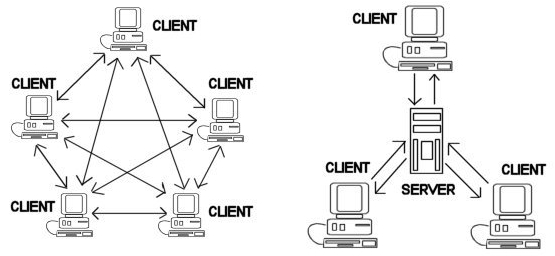
\includegraphics[scale=2.5]{images/p2p_sc.jpg}
\caption{Arquitecturas P2P e Cliente-servidor (respectivamente)}
\end{figure}

\begin{minipage}{1\linewidth}
A nossa opc\c{c}\~ao remeteu para o P2P (de referir ambas eram aplic\'aveis, tinhamos inclusiv\'e exemplos com c\'odigo 
de implementa\c{c}\~ao das duas). O porqu\^e liga-se com o facto de as redes P2P serem um dos sentidos evolut\'ivos das 
redes inform\'aticas. Os jogos acompanham essa evolu\c{c}\~ao sendo emergente cada vez mais jogos em P2P, face \'a 
arquitectura cliente servidor, para o nosso tipo de jogo (Shooters em tempo real FPS por exemplo). Os jogos que 
funcionam em P2P aproveitam melhor os recursos (apesar de ocuparem maior largura de banda) da rede e locais, e s\~ao 
mais tolerantes a falhas. Perdemos no entanto a poss\'ibilidade de implementar uma consider\'avel  quantidade de 
t\'ecnicas de toler\^ancia a falhas, que seriam necess\'arias implementar na arquitectura cliente servidor, por outro 
lado ganhamos em toler\^ancia a falhas nomeadamente quando o servidor c\'ai. Neste caso temos um cliente a tomar o seu 
lugar, conseguimos evitar desta forma a redund\^ancia de servidores de backup. As redes P2P s\~ao tamb\'em muito mais 
simples de implementar (a estructura da rede em si).
\end{minipage}

\subsection{Comunica\c{c}\~ao durante o jogo em rede}

\begin{minipage}{1\linewidth}
A ter em conta que o nosso jogo funciona em P2P em termos de comunica\c{c}\~ao. Cada jogador gere o seu input, envia os 
seus dados a todos os outros jogadores e estes actualizam as suas c\'opias locais deste. Ou seja cada jogador recebe os 
dados de todos os outros jogadores, actualiza as sua c\'opias locais dos mesmos, envia os seus dados a todos os outros e 
desenha tudo (texturas, modeles, etc).
\end{minipage}

\begin{figure}
\centering
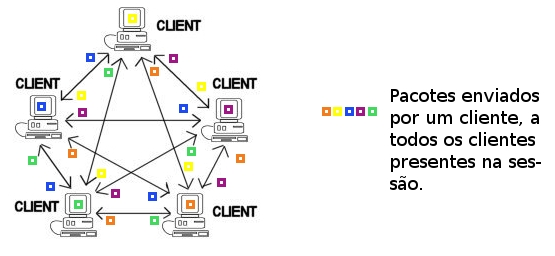
\includegraphics[scale=2.5]{images/game.jpg}
\caption{Comunica\c{c}\~ao durante o jogo}
\end{figure}

\begin{minipage}{1\linewidth} 
Os dados enviados por cada cliente aos restantes s\~ao:
\begin{itemize}
\begin{minipage}{1\linewidth}
\item bool isActive: indica se a nossa nave est\'a activa (estamos vivos?). 
\item Vector3 ship.Position: indica a posi\c{c}\~ao da nossa nave. Um Vector3 \'e um vector de 3 elementos (coordenadas 
X, Y e Z). 
\item Vector3 ship.Velocity: indica a nossa velocidade.
\item float ship.Rotation: indica a rota\c{c}\~ao/orienta\c{c}\~ao da nossa nave. 
\item int Shield: indica o escudo que ainda possuimos.
\item float Radius: indica o raio da nossa nave (ser\'a diferente consoante temos ou n\~ao escudo).
\item int Score: indica a nossa pontua\c{c}\~ao.
\item bool isFiringBullets: indica se estamos a disparar balas.
\item bool isFiringRockets: indica se estamos a disparar misseis.
\item bool isMoving: indica se nos estamos a deslocar/rodar.
\end{minipage}
\end{itemize}

De notar que podiamos emagrecer a comunica\c{c}\~ao enviado booleanos ao inv\'es da velocidade e posi\c{c}\~ao. 
Tornaria-mos desta forma o nosso jogo mais seguro e efici\^ente (n\~ao o tent\'amos mas pretende-mo-lo fazer 
para melhorar este c\'odigo posteriormente a conclus\~ao deste cadeira). 
\end{minipage}
\blankpage

\begin{minipage}{1\linewidth}
N\~ao temos no nosso caso um servidor central a tratar dos dados de todos e a envi\'a-los a cada um dos clientes. O Host \'e um "servidor de sess\~ao", mas n\~ao \'e 
fixo, se ele perder a liga\c{c}\~ao outro cliente toma o seu lugar. O que cada jogador tem \'e um array com uma c\'opia 
dos dados dos outros jogadores (posi\c{c}\~ao, escudo, pontos, etc). Temos ent\~ao aqui a redund\^ancia que vamos 
necessitar de guardar para garantir a manuten\c{c}\~ao do estado de um jogador durante um determinado intervalo, se este 
cair por falha na rede. \\

\end{minipage}

\subsection{Protocolos e QoS}
\begin{minipage}{1\linewidth}
Os nossos pacotes s\~ao UDP sem garantias de recep\c{c}\~ao ou de chegarem por ordem ("SendDataOptions.None" no 
"GamePlayScreen.cs"). A raz\~ao de utilizarmos UDP prende-se com ser o que \'e recomendado em jogos de ac\c{c}\~ao, como 
\'e o nosso ou dos FPS". Isto porque UDP \'e r\'apido e pequenas perdas s\~ao preferiveis a tempos de espera 
indefinidos, resolvendo-se a perda de pacotes com a implementa\c{c}\~ao de sistemas predictivos como t\'ecnica de 
toler\^ancia a falhas. A qualidade de servi\c{c}o \'e assegurada indicando o tempo de m\'edio de "Round trip" nas 
sess\~oes existentes ("qualityOfService.AverageRoundtripTime" na classe "AvailableSessionMenuEntry.cs"), podendo desta 
forma o cliente optar por se juntar a sess\~oes com melhor tempo de resposta (esta opc\c{c}\~ao \'e bastante comun em 
jogos em rede).
\end{minipage}

\subsection{Uso da Plataforma .Net e Xna}
\begin{minipage}{1\linewidth}
A plataforma .Net faculta os mec\^anismos de Threading (as APIs j\'a foram referidas anteriormente), e a plataforma 
XNA estende as funcionalidades da plataforma .Net \'as necessidades especificas de jogos. Em caso de queda de um Host 
\'e referido que \'e escolhido dos menbros dessa sess\~ao um para tomar o lugar de Host, mas nunca \'e especificado
como \'e feita a escolha (\'e algo interno n\~ao indicado, poss\'ivelmente o com melhor liga\c{c}\~ao uma vez que o Xna 
permite analizar a qualidade da rede). A funcionalidade de rede funciona atrav\'es do servi\c{c}o Live da Microsoft que 
entre outras funcionalidades permite sess\~oes de jogos online ou em rede local. O XNA utiliza ainda um servi\c{c}o de 
proxy (XnaLiveProxy), poss\'ivelmente para dar garantias de seguran\c{c}a (ocultar a identidade dos intervinientes na 
sess\~ao). A biblioteca primordial que aqui usamos designa-se por "Microsoft.Xna.Framework.Net", esta \'e respons\'avel 
pelo suporte para Xbox LIVE, multiplayer, e networking. A sua descri\c{c}\~ao pode ser consultada em 
http://msdn.microsoft.com/en-us/library/microsoft.xna.framework.net.aspx. 

\end{minipage}
\blankpage


\section{Conclus\~oes}
\begin{minipage}{1\linewidth}
O XNA \'e uma framework muito completa para desenvolver jogos, no entanto, ainda com alguns pontos fracos muito 
cr\'iticos: \\ \\
\begin{minipage}{1\linewidth}
\begin{itemize}
\item N\~ao suporta OpenGL;
\item N\~ao tem um editor de modelos nativo;
\item N\~ao permite multi-formatos, tendo de ser convertidos na maioria das vezes por n\'os para o som, texturas e 
modelos; \\
\item O XACT em rede apresenta algumas lacunas n\~ao resolvidas; (no entanto em julho sa\'i o XNA 3.0) \\
\item N\~ao (aparentemente) permite gerar execut\'aveis para outras plataformas (Sistemas Operativos); \\
\item N\~ao \'e poss\'ivel correr em computadores sem as bibliotecas do XNA.\\
\end{itemize}
\end{minipage}
Existem numerosos exemplos de c\'odigo mas a sua documenta\c{c}\~ao \'e inexistente e a maioria das vezes a 
integra\c{c}\~ao ou uso destes passa pela sua rescrita o que pretendemos.\\
O .Net torna a cria\c{c}\~ao de aplica\c{c}\~oes para rede muito mais simples de forma r\'apida. 
\end{minipage}
\end{document}